\subsection{Add equations of motion}
Equations of motion:

\begin{align*}
    \Dot v_x &= \frac{F_{3x} + F_{4x} + \left(F_{1x} + F_{2x}\right)\cdot     cos(\delta_f) - \left(F_{1y} + F_{2y}\right)\cdot                    sin(\delta_f)}{m} + r \cdot v_y\\
    \Dot v_y &= \frac{F_{3y} + F_{4y} + \left(F_{1y} + F_{2y}\right)\cdot     cos(\delta_f) + \left(F_{1x} + F_{2x}\right)\cdot                    sin(\delta_f)}{m} - r \cdot v_x\\
    \Dot r &= \frac{-l_2 \cdot \left(F_{3y} + F_{4y}\right)   +   l_1\cdot\left( \left(F_{1x} + F_{2x}\right)\cdot sin(\delta_f) + \left(F_{1y} + F_{2y}\right)\cdot cos(\delta_f) \right)}{I_{zz}}    \\ & + \frac{ \left( \frac{w}{2} \right)\cdot \left( 
F_{4x}-F_{3x} + \left( F_{2x}-F_{1x} \cdot cos(\delta_f) + \left( F_{1y}-F_{2y} \right)\cdot sin(\delta_f) \right)
\right)}{I_{zz}}
\end{align*}


\subsection{Add combined tyre slip}
Force limitation is applied in Matlab so that the longitudinal force for each tire does not exceed $\mu F_z cos(\alpha)$ or go below $-\mu F_z cos(\alpha)$. Then, $F_y$ for each tire is calculated based on the magic tire formula as follows:
\begin{align*}
    F_{y,max} &= \sqrt{(\mu F_z)^2-(F_x)^2}\\
    F_y &= F_{y,max} sin\left( C \cdot atan \left( B \alpha - E \left(B \alpha - atan \left(B \alpha \right)\right)\right)\right)
\end{align*}


\subsection{Test model }
\begin{figure}[H]
      \begin{minipage}[b]{0.5\linewidth}
      \centering
        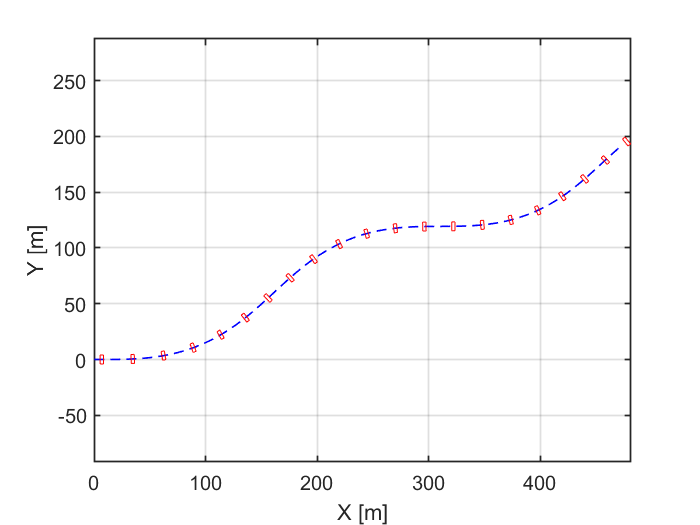
\includegraphics[width=\linewidth]{Figures/1_3_XY.png}
        %  \caption*{Trajectory} 
        % \label{fig:2_4_l}
    \end{minipage} 
    \begin{minipage}[b]{0.5\linewidth}
    \centering
        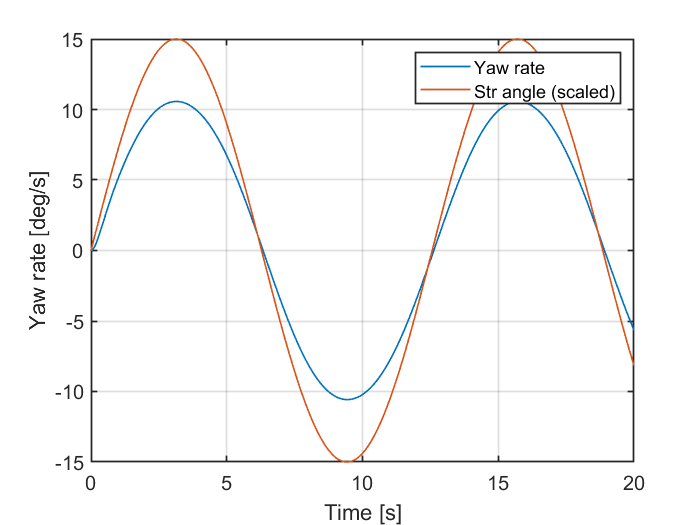
\includegraphics[width=\linewidth]{Figures/1_3_yaw.png}
        % \caption*{Yaw rate}
        % \label{fig:2_4_u}
    \end{minipage} 
    \caption{Base Vehicle Trajectory and Yaw rate for sine wave input}
    %  \label{fig:headbodyrelmotion}
\end{figure}

As seen in the figure above, the vehicle has a sine wave yaw rate, as expected. Since only the equations of motion are implemented, we shouldn't expect any phase shift in the response. And this is clear in the figure above where the peak yaw rate coincides with the peak steering angle input.


\subsection{Check stability in SWD}
For checking the stability of the vehicle, the sine with swell test is carried out in a loop format. The program will start from $60^{\circ}$ up until $300^{\circ}$ or until the vehicle fails one of the specified criteria. The base vehicle in this questions happens to pass all the tests, and hence it is a stable vehicle based on this test.